\documentclass[12pt,a4paper]{article}
\usepackage[polish]{babel}
\usepackage[T1]{fontenc}
\usepackage[utf8x]{inputenc}
\usepackage{hyperref}
\usepackage{url}
\usepackage{graphicx}
\usepackage{listings}
\usepackage{amsmath}
\usepackage{indentfirst}
\usepackage[]{algorithm2e}
\addtolength{\hoffset}{-1.5cm}
\addtolength{\marginparwidth}{-1.5cm}
\addtolength{\textwidth}{3cm}
\addtolength{\voffset}{-1cm}
\addtolength{\textheight}{2.5cm}
\setlength{\topmargin}{0cm}
\setlength{\headheight}{0cm}
\lstset{
  breaklines=true
}
\begin{document}
	
	\title{Dokumentacja projektu\\ Języki Skryptowe}
	\author{Konrad Lubera, gr 1A}
	\date{\today}
	
	\maketitle
	\newpage
	\section*{Część I}
	\subsection*{Opis programu}
	 Projekt spełnia warunki zadania Szyfrowanie Wiadomości z konkursu Algorytmion2015, dodatkowo obsługiwany jest z poziomu powłoki systemu Windows(skrypt batchowski) oraz wyświetla wyniki wykonanych operacji na stronie internetowej. 
	 \\
	\\ Poniżej polecenie z konkursu Algorytmion:
	
	Adam i Janek ustalili między sobą, że każdą wiadomość tekstową, będą szyfrować przy pomocy następującego sposobu:
	\begin{itemize}
	\item   Każdą literę i znak interpunkcyjny należy zamienić na odpowiadającą liczbę kodu ASCII (liczba naturalna od 0 do 127).
	\item Pierwsza, tak powstała liczba, jest zamieniana na system dwójkowy.
	\item Kolejne liczby, wynikające z kodu ASCII, są zamieniane na system liczbowy, który jest równy powiększonej o dwa reszcie z dzielenia przez osiem poprzedniej liczby.
	\item  Ilość cyfr zamienionej liczby, dla każdego systemu liczbowego, wynika z ilości cyfr zamiany liczby maksymalnej, czyli liczby 127 (dla systemu binarnego jest to siedem cyfr). 
	\end{itemize}
	Twoim zadaniem jest napisanie programu, który szyfruje i deszyfruje wiadomości. \\
Szyfrowanie tekstu z pliku tekst.txt do pliku szyfr.txt \\ Deszyfrowanie tekstu z pliku szyfr.txt do pliku odszyfrowane.txt 

	\subsection*{Instrukcja obsługi}
	Aby uruchomić program należy otworzyć plik server.bat znajdujący się w głównym folderze projektu, następnie wybrać opcje Uruchom wpisując 1 na klawiaturze oraz wcisnąć klawisz enter.
		
			
\includegraphics[scale=0.7]{instrukcja}

			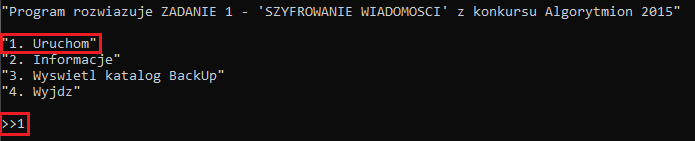
\includegraphics[scale=0.8]{instrukcja2}
	
	
\newpage
	\section*{Część II}
	\subsection*{Część techniczna}
Projekt obsługiwany jest z poziomu powłoki systemu Windows za pomocą pliku server.bat. Za pomocą tego skryptu uruchamiamy cały program, wyświetlamy informacje o projekcie, oraz możemy wyświetlić katalog BackUp. Po wybraniu opcji Uruchom skrypt najpierw tworzy podkatalog backup-dzisiejsza-data w katalogu backup następnie kopiuje tam wszystkie pliki projektu. 


Później uruchamiany jest program server.exe, program ten został napisany w języku Python, plik .exe został wygenerowany za pomocą  aplikacji pyinstaller. Server.exe jest swoistym trzonem całego projektu, tam wykonywane są operacje które spełniają warunki zadania z konkursu Algorytmion2015 tj. odpowiednie szyfrowanie oraz deszyfrowanie słów zapisanych w plikach .txt za pomocą zamiany kodów ASCI poszczególnych liter na odpowiednio obliczone systemy liczbowe oraz późniejszy zapisy wyników wykonanych operacji w plikach .txt, w obsłudze wielu plików pomaga biblioteka glob która została zaimplementowana. Dodatkowo za pomocą biblioteki matplotlib tworzony jest wykres prezentujący  częstotliwość występowania danych systemów liczbowych który zapisywany jest w formacie png w celu późniejszego wykorzystania.

Kolejnym etapem jest uruchomienie przez skrypt server.bat skryptu strona.py. Skrypt ten napisany w języku Python zbiera dane z wszystkich plików które obsługiwał wcześniej program server.exe następnie zapisuje je w pliku storna.html. Zawartość plików .txt jest wyświetlana w formie tabeli według odpowiedniego klucza tj. wejściowe słowo z pliku tekst*.txt jego zaszyfrowany odpowiednik z pliku szyfr*.txt oraz jego zdeszyfrowany odpowiednik z pliku odszyfrowane*.txt. Poniżej tabeli wyświetlany jest obraz który zawiera wcześniej wspominany wykres częstotliwości występowania systemów liczbowych. Ponieważ konieczne było zagregowanie informacji z wielu plików również i przy tworzeniu tego skryptu została wykorzystana biblioteka glob. 


Ostatnim etapem jest uruchomienie pliku strona.html co skutkuje otwarciem przeglądarki i wyświetleniem odpowiednich informacji to ja powstaje ten plik oraz co zawiera zostało opisane w poprzednim akapicie. Za wygląd strony odpowiada pilik kaskadowego arkusza stylów style.css.  

	
	\subsection*{Opis działania} 
Główny algorytm programy szyfruje podane słowa za pomocą zamiany kodu ASCII liter danego słowa z systemu dziesiętnego na odpowiednio wyliczony system liczbowy. Kod pierwszej litery jest zamieniany zawsze na system dwójkowy, system na który zamieniana jest kolejna litera obliczany jest według wzoru: $$sys=(l-1\mod{8})+2$$ 


sys - system liczbowy


l-1 - kod ASCII poprzedniej litery \\

Działanie to jest wykonywane w pętli do końca słowa. Sam algorytm zamiany systemów liczbowych opiszę w następnym rozdziale. Odszyfrowanie słów jest wykonywane przy użyciu tego samego działania.
	\subsection*{Implementacja}
Poniżej implementacja w formie pseudokodu odczytu danych z plików .txt, zapisu danych do pliku .txt, szyfrowania, deszyfrowania słów oraz konwersji systemów liczbowych oraz szyfrowania słów.

	\begin{algorithm}[H]
	\SetKwData{Left}{left}\SetKwData{This}{this}\SetKwData{Up}{up}
	\SetKwInOut{Input}{input}\SetKwInOut{Output}{output}

	\Input{Ścieżka do folderu z plikami .txt}
	\Output{Lista z danymi}
	\BlankLine
	\For{$Pliki w folderze$ \KwTo $Koniec folderu$}{
		\For{$Linia w Pliku$ \KwTo $EOF$}{
		$Lista$=+$Linia w Pliku$}
		}
		\Return $Lista$
		\caption{Odczyt danych z plików}	
	\end{algorithm}
	\begin{algorithm}[H]
	\SetKwData{Left}{left}\SetKwData{This}{this}\SetKwData{Up}{up}
	\SetKwInOut{Input}{input}\SetKwInOut{Output}{output}
	
	\Input{Lista}
	\Output{Pliki .txt}
	\BlankLine
	\For{$ElementListy$ \KwTo $KoniecListy$}{
		\If	{Skończą się elementy dla pliku}{Rozpocznij zapisz w nowym}
		\Else {$KoniecPliku$ = $ElementListy$}
	}
		\caption{Zapis danych do pliku}
	\end{algorithm}
	\newpage
	\begin{algorithm}[H]
		\SetKwData{Left}{left}\SetKwData{This}{this}\SetKwData{Up}{up}
	\SetKwInOut{Input}{input}\SetKwInOut{Output}{output}
	
	\Input{Lista Słów}
	\Output{Zaszyfrowana Lista}
	\For {$ElementListy$ \KwTo $KoniecListy$}{
		\For {$LiterawElementListy$ \KwTo $KoniecElementu$}{
		\tcc{W tym miejscu zamieniany jest system}
		\If {$IndexElementu$ = 0}{ $System$ = 2}
		\Else {$System$ = (($ElementListy-1$ mod 8) +2)}
		\While {$ZamienionyElement$>0}{
			$ZaszyfrowanaLista$+=$ElemementListy$ mod $System$
			$ElementListy$/=$System$		
		}		
		}
		
	}
	\Return Char($ZaszyfrowanaLista$)
		\caption{Szyfrowanie słów}
	\end{algorithm}	
		
	\begin{algorithm}[H]
	\SetKwData{Left}{left}\SetKwData{This}{this}\SetKwData{Up}{up}
	\SetKwInOut{Input}{input}\SetKwInOut{Output}{output}
	
	\Input{Lista Słów (Kody ASCII)}
	\Output{Odszyfrowana Lista}
	\For {$ElementListy$ \KwTo $KoniecListy$}{
		
		\For {$LiterawElementListy$ \KwTo $KoniecElementu$}{
		\tcc{W tym miejscu zamieniany jest system}
		\If {$IndexLiterawElementListy$=0}{$System$=2}
		\Else {$System$ = (Odpowiadający $LiteraWElementOdszyfrowanaLista$-1 mod 8)+2}
		$OdszyfrowanyElemnt$ = $LiterawElementListy$*Pow($System$,$IndexElementListy$)
		\BlankLine
		\If {$OdszyfrowanyElemnt$>127}{$OdszyfrowanyElemnt$-=127}
		$OdszyfrowanaLista$+=$OdszyfrowanyElemnt$
		}
	}
	Odwróć($OdszyfrowanaLista$)
	
	\Return Char($OdszyfrowanaLista$)
		\caption{Odszyfrowanie słów}
	\end{algorithm}	
	\newpage
	\section*{Pełen kod programu}

	\begin{itemize}
	\item SERVER.BAT
	\begin{lstlisting}
@echo off
title Projekt Semestralny Jezyki Skryptowe

:main
cls
echo.
echo "Program rozwiazuje ZADANIE 1 - 'SZYFROWANIE WIADOMOSCI' z konkursu Algorytmion 2015"
echo.
echo "1. Uruchom"
echo "2. Informacje"
echo "3. Wyswietl katalog BackUp"
echo "4. Wyjdz"
echo.
set /p op=">>"
if %op%==1 goto start 
if %op%==2 goto info
if %op%==3 goto backup
if %op%==4 goto koniec

:start
mkdir .\backup\backup_%date%
xcopy /Q /Y strona.html .\backup\backup_%date%
xcopy /Q /Y style.css .\backup\backup_%date%
xcopy /Q /Y strona.py .\backup\backup_%date%
xcopy /Q /Y server.py .\backup\backup_%date%
xcopy /Q /Y .\input .\backup\backup_%date%
xcopy /Q /Y .\output .\backup\backup_%date%
start server.exe
start strona.py
start strona.html
goto koniec

:info
cls 
echo "Projekt Semstralny z przedmiotu Jezyki Skryptowe"
echo " ZADANIE 1 - 'SZYFROWANIE WIADOMOSCI' z konkursu Algorytmion 2015"
echo.
echo "Konrad Lubera"
echo "Informatyka sem III grupa 1A, RMS"
pause
goto main

:backup
cls
dir .\backup /W
pause
goto main

:koniec
pause
echo on

	\end{lstlisting}
	
	\item SERVER.PY
	\begin{lstlisting}[language=Python]
import matplotlib.pyplot as plt
import glob

systems ={}


def fread(nazwa):
    path = nazwa
    files = glob.glob(path)
    i = 0
    list = []
    for name in files:
        list.append([])
        with open(name, 'r') as f:
            list[i] = f.readlines()
            f.close()
        i+=1
    return list

def read(n):
    list = []
    path = n
    files = glob.glob(path)
    word = ''
    i = 0
    j = 0
    for name in files:
        list.append([])
        with open(name, 'r') as f:
            for line in f:
                list[j].append([])
                for letter in line:
                    if letter == ' ':
                        list[j][i].append(word)
                        word = ''
                    elif letter=="\n": pass
                    else:
                        word+=letter
                i += 1
            f.close()
        i = 0
        j += 1
    return list


def fwrite(name, list):
    for c in range(len(list)):
        path = name
        path = path + str(c) + '.txt'
        file = open(path, 'w')
        for i in range(len(list[c])):
            for j in range(len(list[c][i])):
                for n in range(len(list[c][i][j])):
                    file.write(str(list[c][i][j][n]))
                    if n == len(list[c][i][j]) - 1:
                        file.write(" ")
                if j == len(list[c][i]) - 1:
                    file.write('\n')
        file.close()



def write(name, list):
    for i in range(len(list)):
        path = name
        path = path + str(i) + '.txt'
        file = open(path, 'w')
        for item in list[i]:
            file.write(item +'\n')
        file.close()

def encrypt(list_encrypt):
    encrypted = []
    for c in range(len(list_encrypt)):
        encrypted.append([])
        for i in range(len(list_encrypt[c])):
            encrypted[c].append([])
            for j in range(len(list_encrypt[c][i])):
                if list_encrypt[c][i][j] != '\n':
                    if j != 0:
                        sys = (ord(list_encrypt[c][i][j - 1]) % 8) + 2
                        if sys not in systems: systems.update({sys: 1})
                        else: systems[sys]+=1
                        encrypted[c][i].append(conv_to_sys(ord(list_encrypt[c][i][j]), sys))

                    else:
                        if 2 not in systems: systems.update({2: 1})
                        else: systems[2] += 1
                        encrypted[c][i].append(conv_to_sys(ord(list_encrypt[c][i][j]), 2))
    fwrite("output/szyfr", encrypted)


def conv_to_sys(number, system):
    converted = []
    n = number
    s = system
    while n > 0:
        converted.append(n % s)
        n = int(n / s)
    converted.reverse()
    return converted


def conv_from_sys(number, sys):
    sum = 0
    num = ''.join(reversed(number))
    for i in range(len(num)):
        sum+=int(num[i]) * pow(sys,i)
    if sum>127: sum-=127
    return sum


def decrypt(list):
    decrypted = []
    sys = 0
    word=''
    letter=0
    for c in range(len(list)):
        decrypted.append([])
        for i in range(len(list[c])):
            for j in range(len(list[c][i])):
                if j==0: sys=2
                letter = conv_from_sys(list[c][i][j], sys)
                word+=chr(letter)
                sys = (letter%8)+2
            decrypted[c].append(word)
            word =''
    write("output/odszyfrowane",decrypted)

def plot():
    fig, ax = plt.subplots()
    plt.bar(systems.keys(),systems.values(),color="forestgreen")
    plt.title("Ilosc wystapien danego systemu liczbowego" )
    plt.xlabel("Rodzaj systemu")
    plt.ylabel("Ilosc wystapien")
    plt.savefig("images/plot.png",dpi=100)



encrypt(fread("input/*.txt"))
decrypt(read("output/szyfr*.txt"))
plot()

	\end{lstlisting}
	
	\item STRONA.PY
	\begin{lstlisting}[language=Python]
import glob

html = open("strona.html", 'w')

path_1 = "input/*.txt"
path_2 = "output/szyfr*.txt"
path_3 = "output/odszyfrowane*.txt"
files_1 = glob.glob(path_1)
files_2 = glob.glob(path_2)
files_3 = glob.glob(path_3)

words = []
encrypted = []
decrypted = []

for name in files_1:
    with open(name) as f:
        word = f.readlines()
        words += word
        f.close()


for name in files_2:
    with open(name) as f:
        word = f.readlines()
        encrypted += word
        f.close()

for name in files_3:
    with open(name) as f:
        word = f.readlines()
        decrypted += word
        f.close()
        
html.write('<!DOCTYPE HTML>\n'
           '<html lang="pl">\n<head>'
           '    <meta charset="utf-8" />\n'
           '    <title>Jezyki Skryptowe Projekt</title>\n'
           '    <meta name="descripton" content="Projekt semestralny Jezyki Skryptowe Konrad Lubera"/>\n'
           '    <meta http-equiv="X-UA-Compatible" content="IE=edge,chrome=1"/> \n'
           '    <link rel="stylesheet" href="style.css" type="text/css" /> \n'
           '    <link href="https://fonts.googleapis.com/css?family=Lato&display=swap" rel="stylesheet"> \n'
           '</head> \n'
           '<body> \n'
           '    <div id="container"> \n'
           '        <div id="header"> \n'
           '         "Szyfrowanie wiadomosci" - Algorytmion 2015 \n         </div> \n'
           '        <div id="content"> \n'
           '            <div id="tab">\n'
           '            <table>\n'
           '                 <tr>\n'
           '                     <th>tekst.txt</th>\n'
           '                     <th>szyfr.txt</th>\n'
           '                     <th>odszyfrowane.txt</th>\n'
           '                 </tr>\n')
i = 0
j = 0
n = 0
while (i != len(words)) and (j != len(encrypted)) and (n != len(decrypted)):
            html.write('                 <tr>\n                     <td>')
            html.write(words[i].replace('\n',''))
            html.write('</td>\n                     <td>')
            html.write(encrypted[j].replace('\n',''))
            html.write('</td>\n                     <td>')
            html.write(decrypted[n].replace('\n', ''))
            html.write('</td> \n                 </tr>\n')
            i+=1
            j+=1
            n+=1
html.write('             </table>\n'
           '             </div>\n'
           '            <div id="txt">Ponizej zestwaienie czestowliwosci wystepowania danych systemow liczbowych </div> \n'
           '            <img src="images\plot.png"/>\n'           
           '        </div> \n'
           '           <div id="footer"> \n'
           '            &copy Konrad Lubera, RMS POLSL \n'
           '           </div> \n'
           '    </div> \n'
           '</body> \n'
           )
html.close()

	\end{lstlisting}
	
	\item STRONA.HTML
	\begin{lstlisting}[language=Html]
<!DOCTYPE HTML>
<html lang="pl">
<head>    <meta charset="utf-8" />
    <title>Jezyki Skryptowe Projekt</title>
    <meta name="descripton" content="Projekt semestralny Jezyki Skryptowe Konrad Lubera"/>
    <meta http-equiv="X-UA-Compatible" content="IE=edge,chrome=1"/> 
    <link rel="stylesheet" href="style.css" type="text/css" /> 
    <link href="https://fonts.googleapis.com/css?family=Lato&display=swap" rel="stylesheet"> 
</head> 
<body> 
    <div id="container"> 
        <div id="header"> 
         "Szyfrowanie wiadomosci" - Algorytmion 2015 
         </div> 
        <div id="content"> 
            <div id="tab">
            <table>
                 <tr>
                     <th>tekst.txt</th>
                     <th>szyfr.txt</th>
                     <th>odszyfrowane.txt</th>
                 </tr>
                 <tr>
                     <td>REPUBLIKA</td>
                     <td>1010010 1011 143 1010101 123 1030 201 2210 230 </td>
                     <td>REPUBLIKA</td> 
                 </tr>
                 <tr>
                     <td>NIEZAWODNY</td>
                     <td>1001110 111 2120 156 1001 10020 87 75 210 131 </td>
                     <td>NIEZAWODNY</td> 
                 </tr>
                 <tr>
                     <td>OSZOLOMIENIE</td>
                     <td>1001111 102 330 1033 84 211 85 133 2120 141 111 2120 </td>
                     <td>OSZOLOMIENIE</td> 
                 </tr>
                 <tr>
                     <td>ANTYK</td>
                     <td>1000001 2220 124 225 2210 </td>
                     <td>ANTYK</td> 
                 </tr>
                 <tr>
                     <td>UPRZEJMY</td>
                     <td>1010101 143 1010010 1122 1011 134 1031 155 </td>
                     <td>UPRZEJMY</td> 
                 </tr>
                 <tr>
                     <td>PIASEK</td>
                     <td>1010000 1001001 2102 10002 234 135 </td>
                     <td>PIASEK</td> 
                 </tr>
                 <tr>
                     <td>NAUCZYCIEL</td>
                     <td>1001110 101 10011 124 330 1121 2111 243 2120 136 </td>
                     <td>NAUCZYCIEL</td> 
                 </tr>
                 <tr>
                     <td>BALKON</td>
                     <td>1000010 1001 2211 203 304 86 </td>
                     <td>BALKON</td> 
                 </tr>
                 <tr>
                     <td>CZYTANIE</td>
                     <td>1000011 330 1121 10010 145 2220 111 2120 </td>
                     <td>CZYTANIE</td> 
                 </tr>
                 <tr>
                     <td>WSPARCIE</td>
                     <td>1010111 102 310 1000001 10001 1003 243 2120 </td>
                     <td>WSPARCIE</td> 
                 </tr>
                 <tr>
                     <td>ZWYCIEZCA</td>
                     <td>1011010 1113 108 2111 243 2120 156 1003 230 </td>
                     <td>ZWYCIEZCA</td> 
                 </tr>
                 <tr>
                     <td>LATAWIEC</td>
                     <td>1001100 145 10010 145 10020 81 2120 124 </td>
                     <td>LATAWIEC</td> 
                 </tr>
                 <tr>
                     <td>SIEDZENIE</td>
                     <td>1010011 243 2120 125 230 1011 141 111 2120 </td>
                     <td>SIEDZENIE</td> 
                 </tr>
                 <tr>
                     <td>SYSTEM</td>
                     <td>1010011 324 10002 314 153 140 </td>
                     <td>SYSTEM</td> 
                 </tr>
                 <tr>
                     <td>WKURZENIE</td>
                     <td>1010111 83 320 145 1122 1011 141 111 2120 </td>
                     <td>WKURZENIE</td> 
                 </tr>
                 <tr>
                     <td>OKNO</td>
                     <td>1001111 83 303 117 </td>
                     <td>OKNO</td> 
                 </tr>
                 <tr>
                     <td>GENERAL</td>
                     <td>1000111 76 141 105 145 1001 2211 </td>
                     <td>GENERAL</td> 
                 </tr>
                 <tr>
                     <td>OSIEDLE</td>
                     <td>1001111 102 243 2120 125 204 153 </td>
                     <td>OSIEDLE</td> 
                 </tr>
                 <tr>
                     <td>NOC</td>
                     <td>1001110 117 74 </td>
                     <td>NOC</td> 
                 </tr>
                 <tr>
                     <td>LOTNIK</td>
                     <td>1001100 211 103 210 111 2210 </td>
                     <td>LOTNIK</td> 
                 </tr>
                 <tr>
                     <td>ZOO</td>
                     <td>1011010 1033 87 </td>
                     <td>ZOO</td> 
                 </tr>
                 <tr>
                     <td>WAKACJE</td>
                     <td>1010111 72 2210 230 2111 244 1011 </td>
                     <td>WAKACJE</td> 
                 </tr>
                 <tr>
                     <td>BEZTROSKA</td>
                     <td>1000010 1011 156 1110 214 1033 102 300 230 </td>
                     <td>BEZTROSKA</td> 
                 </tr>
                 <tr>
                     <td>PIEPRZ</td>
                     <td>1010000 1001001 2120 143 1010010 1122 </td>
                     <td>PIEPRZ</td> 
                 </tr>
                 <tr>
                     <td>BILANS</td>
                     <td>1000010 1021 2211 145 2220 123 </td>
                     <td>BILANS</td> 
                 </tr>
                 <tr>
                     <td>MALPA</td>
                     <td>1001101 122 2211 212 1000001 </td>
                     <td>MALPA</td> 
                 </tr>
                 <tr>
                     <td>LOKOWKI</td>
                     <td>1001100 211 83 304 106 83 243 </td>
                     <td>LOKOWKI</td> 
                 </tr>
                 <tr>
                     <td>PARASOL</td>
                     <td>1010000 1000001 10001 1001 10002 304 84 </td>
                     <td>PARASOL</td> 
                 </tr>
                 <tr>
                     <td>KOMBINERKI</td>
                     <td>1001011 304 85 123 1021 2220 105 145 1023 243 </td>
                     <td>KOMBINERKI</td> 
                 </tr>
                 <tr>
                     <td>PLAKAT</td>
                     <td>1010000 1001100 145 2210 230 10010 </td>
                     <td>PLAKAT</td> 
                 </tr>
             </table>
             </div>
            <div id="txt">Ponizej zestwaienie czestowliwosci wystepowania danych systemow liczbowych </div> 
            <img src="images\plot.png"/>
        </div> 
           <div id="footer"> 
            &copy Konrad Lubera, RMS POLSL 
           </div> 
    </div> 
</body> 
	\end{lstlisting}
	
	\item STYLE.CSS
	\begin{lstlisting}
body
{
    margin: 0 !important;
    background-color: rgb(65, 62, 62);
    font-family: 'Lato', sans-serif;
    
}
table
{
    width: 100%;
    border-collapse: collapse;
    margin-left: auto;
    margin-right: auto;
    border: 3px solid rgb(218, 217, 217);
}
td, th
{
    padding: 8px;
    border: 1px solid rgb(218, 217, 217);
    
}
th
{
    text-align: center;
    border-bottom: 3px solid rgb(218, 217, 217);
    background-color:  rgb(31, 102, 22);
}
td
{
    text-align: left;
}
tr:hover {background-color: #636363;} 
#tab
{
    padding: 15px;
    margin-left: auto;
    margin-right: auto;
    overflow-x: auto;
}
#container
{
    width: 100%;
    
}
#header
{
    
    width: 100%;
    padding: 15px 0;
    background-color: rgb(39, 128, 27);
    color: whitesmoke;
    text-align: center;
    font-size: 20px;
    border-top: 5px solid  rgb(31, 102, 22);
    border-bottom: 5px solid  rgb(31, 102, 22);

}
#content
{
    min-height: 905px;
    width: 1000px;
    margin-left: auto;
    margin-right: auto;
    text-align: justify;
    
    background-color: rgb(73, 73, 73);
    color: whitesmoke;
    
}

#footer
{
   
    text-align: center;
    color: whitesmoke;
    padding: 10px;
    background-color: rgb(54, 54, 54);
}
#txt
{
    font-size: 20px;
    text-align: center;
    padding-bottom: 15px ;
}

img {
    display: block;
    margin-left: auto;
    margin-right: auto;
    padding-bottom: 15px;
  }
	\end{lstlisting}
	\end{itemize}

\end{document}
